\documentclass[a4paper]{article}

% Set for specific document
\def\DOCTITLE{CSC3423 Biocomputing Coursework Report}
\def\DOCAUTHOR{Dan Nixon (120263697)}
\def\DOCDATE{\today}

% Set document attributes
\title{\DOCTITLE}
\author{\DOCAUTHOR}
\date{\DOCDATE}

\usepackage{fullpage}
\usepackage{scrextend}
\usepackage{titlesec}
\usepackage{fancyhdr}
\usepackage{hyperref}
\usepackage[style=numeric-comp,natbib=true]{biblatex}
\usepackage{booktabs}

\addbibresource{DanNixon_CSC3423_Report.bib}

% Handle graphics correctly
\ifx\pdftexversion\undefined
\usepackage{graphicx}
% \usepackage[dvips]{graphicx}
\else
\usepackage[pdftex]{graphicx}
\DeclareGraphicsRule{*}{mps}{*}{}
\fi

% Setup headers and footers
\pagestyle{fancy}
\lhead{}
\chead{\DOCTITLE}
\rhead{}
\rfoot{\DOCDATE}
\cfoot{\thepage}
\lfoot{\DOCAUTHOR}

% New page for each section
\newcommand{\sectionbreak}{\clearpage}

% Set header and footer sizes
\renewcommand{\headrulewidth}{0.4pt}
\renewcommand{\footrulewidth}{0.4pt}
\setlength{\headheight}{15.2pt}
\setlength{\headsep}{15.2pt}

\begin{document}

\maketitle

\begin{abstract}
  This report will give an overview of the two nature inspired algorithms that
  were implemented to solve the classification problem, how they differ from
  what was outlined in the proposal and a critical evaluation between the
  performance of both in terms of learning time and classification accuracy.
\end{abstract}

\section{Genetic Algorithm}
\label{sec:ga}

A genetic algorithm is a very simple nature inspired algorithm that can be
applied to a wide range of problems providing that the fitness of a candidate
solution can be evaluated.

In the case of this classification problem the fitness function is simply the
percentage of correctly classified points within the bounds of the classifier.

\subsection{Implementation}
\label{sec:ga_implementation}

The implementation of the genetic algorithm mostly follows what was described in
the proposal document however with several important changes that were required
as part of an optimisation or technical limitation.

The first notable change is the data format of the knowledge representation,
previously this would have stored an "origin" point and a length in each
dimension to denote the bounds of the hyperrectangle.

In the final implementation this has been changed to storing two points
diagonally opposite from each other as shown in figure \ref{fig:ga_kr}, this was
due to an optimisation that allowed the values of the genes that represented the
coordinates of each point to be constrained between two values, this was done to
limit the search space the mutations of a new classifier would operate within in
order to converge to the best solution faster.

This optimisation simply performs a linear search through each \texttt{Instance}
of the training \texttt{InstanceSet} in order to obtain the minimum and maximum
values for each dimension and then sets the limits of the relevant
\texttt{DoubleGene} to these values plus a padding constant.

\begin{figure}[h!]
  \centering
  \includegraphics[width=0.4\textwidth]{out/ga_kr.eps}
  \caption{3D hyperrectangle classifier}
  \label{fig:ga_kr}
\end{figure}

It was also my intention to add validation to the \texttt{CompositeGene} which
would hold the upper and lower positions of a single dimension, however instead
of generating a new mutation on a failed validation the JGAP framework instead
aborted the entire evolution step.

The implementation of the genetic algorithm was done using the JGAP \cite{jgap}
Java library, the structure of the code the was used to integrate this into the
provided framework is shown in figure \ref{fig:ga_uml}.

\begin{figure}[h!]
  \centering
  \includegraphics[width=0.9\textwidth]{out/ga_uml.1}
  \caption{Genetic algorithm implementation UML diagram}
  \label{fig:ga_uml}
\end{figure}

The \texttt{HyperrectangleFrame} class is used to provide a visualisation of the
progress of the algorithm, after the learning process completes the classifier
is plotted over the training data as shown in figure \ref{fig:ga_vis}.

\begin{figure}[h!]
  \centering
  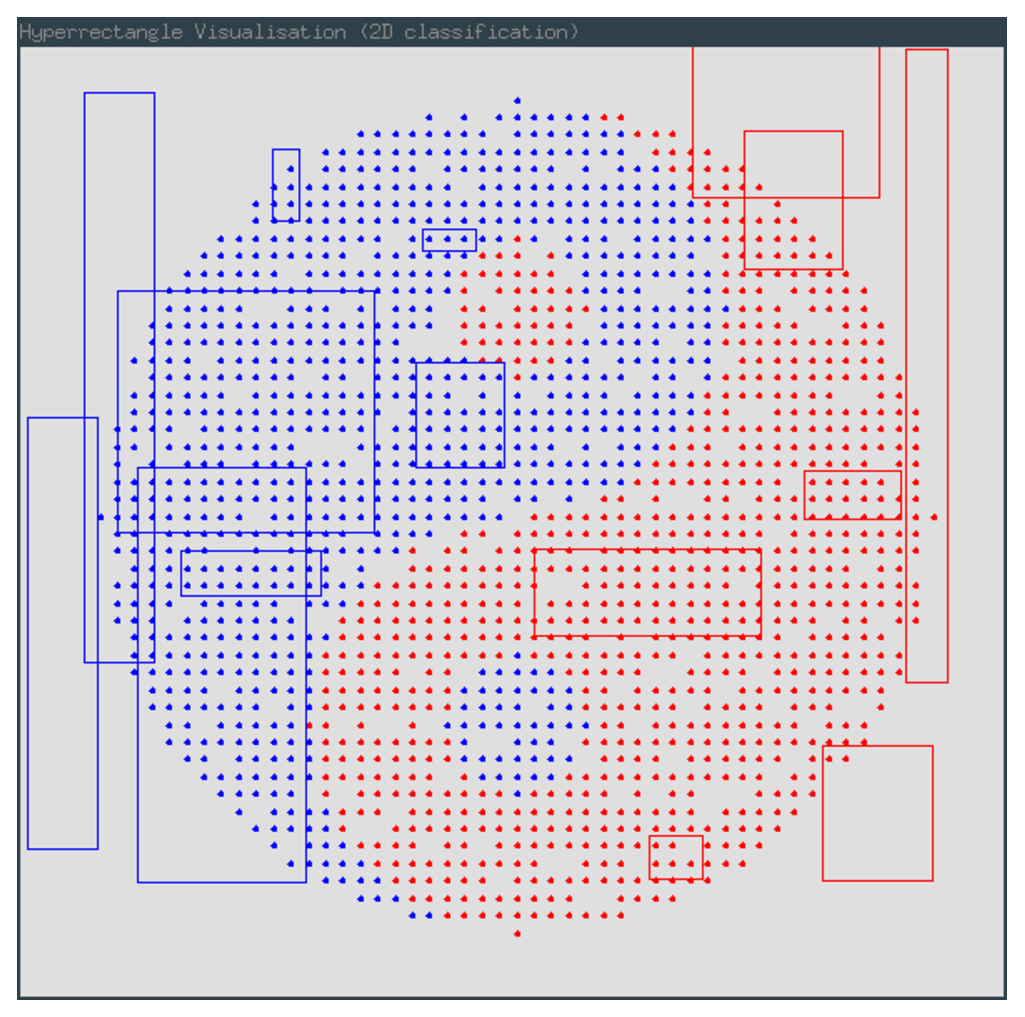
\includegraphics[width=0.6\textwidth]{graphics/ga_vis.eps}
  \caption{Genetic algorithm visualisation}
  \label{fig:ga_vis}
\end{figure}

The final implementation uses a selection algorithm that selects the top
chromosomes based on their fitness value, this selection algorithm operates by
selecting the best $n$ chromosomes from the current population to go forth to
the population of the next iteration where $n$ is given by:

\[
  n = s * p;
\]

where $s$ is the population size and $p$ is an attribute of the system.

This differs from the original proposal to use tournament selection for reasons
described in section \ref{sec:ga_tuning}.

The crossover algorithm used is the default provided by the JGAP
\texttt{DefaultConfiguration}. This algorithm selects two chromosomes for
crossover, selects a gene at random and swaps that gene and all genes after
between the two chromosomes.

This crossover operation is performed $1/c$ times where $c$ is the crossover
rate, by default this is 0.35.

The mutation algorithm used is the default provided by the JGAP
\texttt{DefaultConfiguration}. This mutation algorithm mutates a given
percentage of the chromosomes in the population, by default this mutation rate
is a constant of $1/12$ of the population size.

The actual mutation performed is simple an offset by a random value between the
upper and lower bounds of the gene value.

When the best chromosome for a classifier is found it is converted to
coordinates for the hyperrectangle and a classification value by the
\texttt{updateFromChromosome()} function.

Classification in the \texttt{classifyInstance()} function is performed by
checking if the coordinates of the \texttt{Instance} being classified falls
within the bounds of the hyperrectangle, if so the instance is classified based
on the classification value given to this classifier during the learning phase,
otherwise the instance is unclassified.

\subsection{Tuning}
\label{sec:ga_tuning}

I selected three important parameters to be tuned in the genetic algorithm
implementation; the population size, the target accuracy for each classifier
(i.e. the accuracy required for the learning process to terminate) and the
selection algorithm being used.

Several parameters were kept constant for all tests, these parameters are:

\begin{description}
  \item[Maximim learning iterations (100)] \hfill \\
    The maximum number of iterations to be executed in the learning process.
  \item[Crossover operator] \hfill \\
    The crossover algorithm as described in section \ref{sec:ga_implementation}.
  \item[Mutation operator] \hfill \\
    The mutation algorithm as described in section \ref{sec:ga_implementation}.
\end{description}

The values used in the tests and the results are given in table
\ref{tab:ga_tuning}. In each test 10 runs of the algorithm were performed and
the values recorded are the results that show the best time and accuracy.

\begin{table}[h!]
  \centering
  \begin{tabular}{@{}lllllll@{}}
    \toprule
    Population Size & Target (\%) & Selector       & Accuracy (\%) & Error (\%) & Unclassified (\%) & Time (s) \\
    \midrule
    100             & 0.9         & Best (0.9)     & 95.26         & 4.74       & 0                 & 23.96    \\
    100             & 0.95        & Best (0.9)     & 97.37         & 2.63       & 0                 & 33.622   \\
    100             & 0.99        & Best (0.9)     & 95.79         & 4.21       & 0                 & 46.085   \\
    20              & 0.9         & Best (0.9)     & 94.21         & 5.79       & 0                 & 14.269   \\
    20              & 0.95        & Best (0.9)     & 94.74         & 5.26       & 0                 & 19.23    \\
    20              & 0.99        & Best (0.9)     & 95.79         & 4.21       & 0                 & 23.143   \\
    200             & 0.9         & Best (0.9)     & 95.26         & 4.21       & 0.53              & 56.417   \\
    200             & 0.95        & Best (0.9)     & 94.21         & 5.79       & 0                 & 60.465   \\
    200             & 0.99        & Best (0.9)     & 94.74         & 5.26       & 0                 & 73.05    \\
    100             & 0.9         & Tournament (2) & 95.79         & 4.21       & 0                 & 53.039   \\
    100             & 0.95        & Tournament (2) & 95.79         & 4.21       & 0                 & 67.503   \\
    100             & 0.99        & Tournament (2) & 96.84         & 3.16       & 0                 & 93.144   \\
    20              & 0.9         & Tournament (2) & 94.21         & 5.26       & 0.53              & 35.135   \\
    20              & 0.95        & Tournament (2) & 96.32         & 3.68       & 0                 & 50.156   \\
    20              & 0.99        & Tournament (2) & 91.58         & 8.42       & 0                 & 32.734   \\
    200             & 0.9         & Tournament (2) & 94.74         & 5.26       & 0                 & 77.3     \\
    200             & 0.95        & Tournament (2) & 96.32         & 3.68       & 0                 & 83.885   \\
    200             & 0.99        & Tournament (2) & 95.79         & 4.21       & 0                 & 100.731  \\
    100             & 0.9         & Tournament (5) & 95.26         & 4.74       & 0                 & 66.057   \\
    100             & 0.95        & Tournament (5) & 96.32         & 3.68       & 0                 & 82.002   \\
    100             & 0.99        & Tournament (5) & 95.79         & 3.68       & 0.53              & 106.346  \\
    20              & 0.9         & Tournament (5) & 93.16         & 6.84       & 0                 & 37.7     \\
    20              & 0.95        & Tournament (5) & 94.21         & 5.79       & 0                 & 49.235   \\
    20              & 0.99        & Tournament (5) & 89.47         & 10.53      & 0                 & 41.093   \\
    200             & 0.9         & Tournament (5) & 95.79         & 4.21       & 0                 & 138.576  \\
    200             & 0.95        & Tournament (5) & 94.21         & 5.79       & 0                 & 103.349  \\
    200             & 0.99        & Tournament (5) & 95.79         & 4.21       & 0                 & 129.103  \\
    \bottomrule
  \end{tabular}
  \caption{Genetic algorithm tuning}
  \label{tab:ga_tuning}
\end{table}

These results show that the most optimal solution in terms of classification
accuracy was obtained using a population size of 100, a target classification
accuracy of 95\% and the best chromosome selection algorithm.

There is a notable speed increase with only a small reduction in classification
accuracy when using a smaller population size, 20 in this case. However I chose
to favour classification accuracy in the selection of parameters for the final
implementation.

It is clear to see that the use of the best chromosome selector gives a
noticeable speed increase over tournament selection. This could be due to the
increased favour of exploitation that the best chromosome selector provides by
taking only the best chromosomes from the population as opposed to tournament
selection where due to the fact that the choice of chromosomes that take part in
one tournament is random, there is still a chance that a chromosome with poor
fitness can be put forward to the next population.

\section{Neural Network}
\label{sec:nn}

TODO: reason for selection

\subsection{Implementation}
\label{sec:nn_implementation}

The neural network was implemented using the Neuroph \cite{neuroph} Java
library, the code structure of the implementation is shown in figure
\ref{fig:nn_uml}.

The implementation uses the \texttt{MultiLayerPerceptron} class from Neuroph
which implements a standard multi layer perceptron network in which all neurons
in a given layer connect to all nodes in their neighbouring layers and the
network is strictly feed forward.

The network is trained using back propagation which is the default learning
algorithm for this network type within Neuroph.

\begin{figure}[h!]
  \centering
  \includegraphics[width=0.9\textwidth]{out/nn_uml.1}
  \caption{Neural network implementation UML diagram}
  \label{fig:nn_uml}
\end{figure}

The \texttt{NNLearnListener} class is used for progress reporting during the
learning process and also updates the network visualisation if it is enabled.
The progress reporting outputs the iteration number and classification error on
the training data for each iteration.

The \texttt{NeuralNetworkFrame} class is used to provide a visualisation of the
neural network during the learning process, this plots the network as a graph
where the colour of the connecting arc is determined by the weight associated
with it in the network.

The neurons are colour coded; green are the input layer, blue are inner layers
and red is the output layer. Bias neurons are a hollow circle.

\begin{figure}[h!]
  \centering
  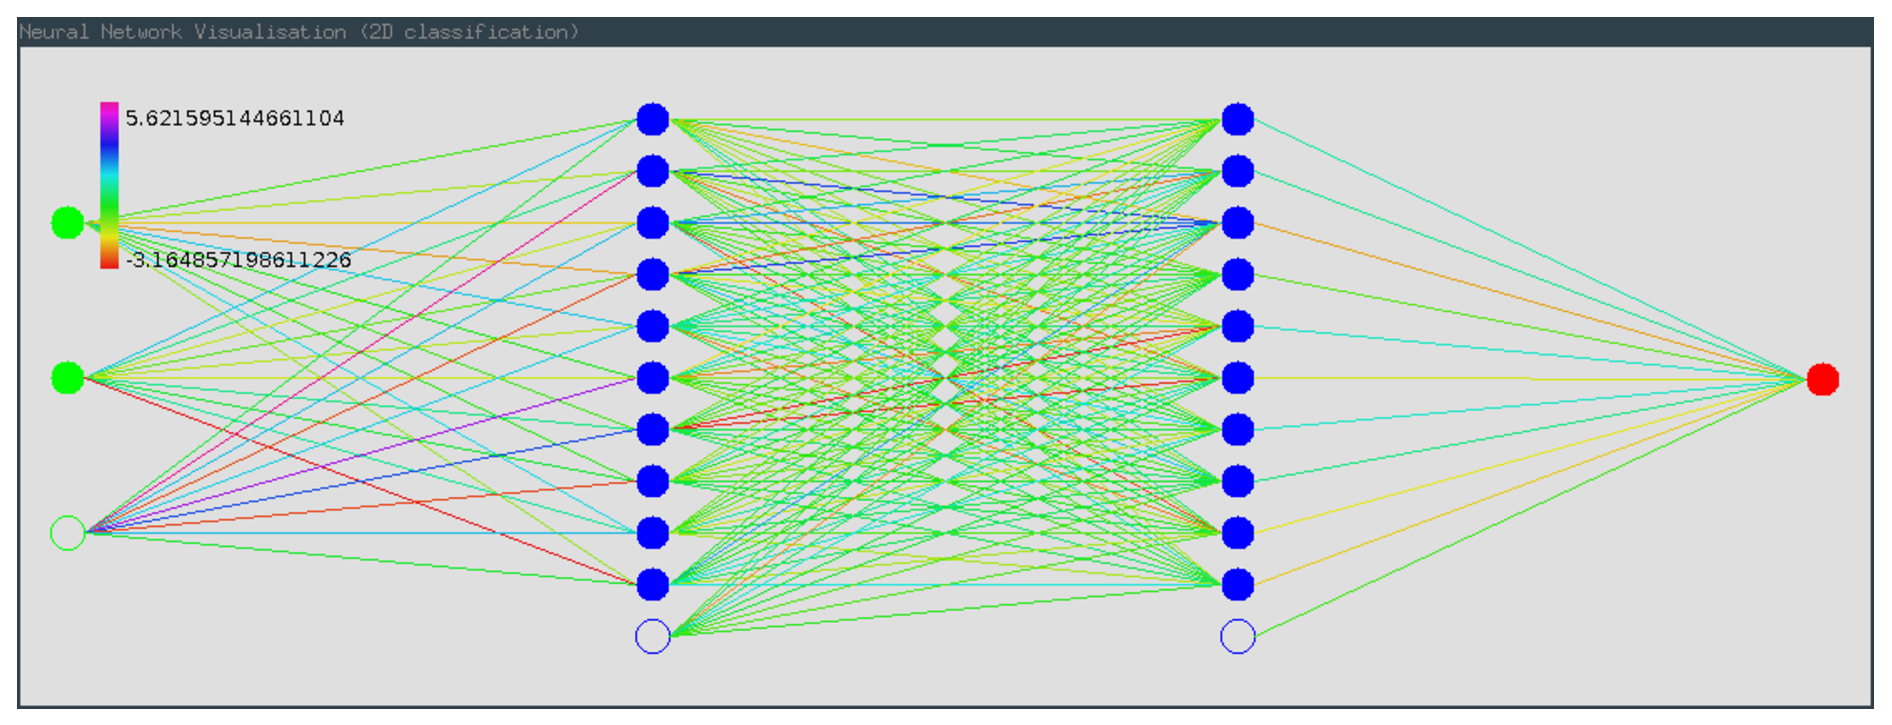
\includegraphics[width=0.8\textwidth]{graphics/nn_vis.eps}
  \caption{Neural network visualisation}
  \label{fig:nn_vis}
\end{figure}

Classification in the \texttt{classifyInstance()} function is performed by
simply setting the input layer of the trained network based on the attributes of
the instance being classified and obtaining the output value. Due to the
functional form of a neural network all instances will always be classified.

In order to convert between the \texttt{Instance} data type in the provided
framework and a suitable data type for Neuroph there is a utility function,
\texttt{instanceToRow()}, which converts and \texttt{Instance} to a
\texttt{DataSetRow} which when part of a \texttt{DataSet} can be used to train
the network.

\subsection{Tuning}
\label{sec:nn_tuning}

TODO

\begin{table}[h!]
  \centering
  \begin{tabular}{@{}lllllll@{}}
    \toprule
    Transfer Function  & Topology     & Learning Rate & Accuracy (\%) & Error (\%) & Unclassified (\%) & Time (s)   \\
    \midrule
    Sigmoid            & 2, 5, 1      & 0.01          & 91.05         & 8.95       & 0                 & 14.075     \\
    Hyperbolic Tangent & 2, 5, 1      & 0.01          & 92.63         & 7.37       & 0                 & 14.396     \\
    Sigmoid            & 2, 10, 1     & 0.01          & 83.68         & 16.32      & 0                 & 22.149     \\
    Hyperbolic Tangent & 2, 10, 1     & 0.01          & 94.74         & 5.26       & 0                 & 25.602     \\
    Sigmoid            & 2, 20, 20, 1 & 0.01          & 97.37         & 2.63       & 0                 & 11.453     \\
    Hyperbolic Tangent & 2, 20, 20, 1 & 0.01          & 97.37         & 2.63       & 0                 & 7.098      \\
    Sigmoid            & 2, 20, 10, 1 & 0.01          & 97.37         & 2.63       & 0                 & 6.355      \\
    Hyperbolic Tangent & 2, 20, 10, 1 & 0.01          & 97.37         & 2.63       & 0                 & 2.667      \\
    Sigmoid            & 2, 10, 10, 1 & 0.01          & 92.11 (1)     & 7.89 (1)   & 0                 & 63.059 (1) \\
    Hyperbolic Tangent & 2, 10, 10, 1 & 0.01          & 97.37         & 2.63       & 0                 & 3.728      \\
    \bottomrule
  \end{tabular}
  \caption{Neural network tuning}
  \label{tab:nn_tuning}
\end{table}

TODO

\section{Comparison of algorithms}
\label{sec:comparison}

A comparison between the performance of the two algorithms, both in terms of the
time taken for learning and the accuracy of the resulting classification was
performed using a dataset of 100 runs of each algorithm using the optimal
parameters found in sections \ref{sec:ga_tuning} and \ref{sec:nn_tuning}.

Statistics of the results of this performance test are shown in table
\ref{tab:comparison_avg}, in the case of iteration count for the genetic
algorithm the total number of iterations over all classifiers is given with the
number of classifiers shown in brackets.

\begin{table}[h!]
  \centering
  \begin{tabular}{@{}lll@{}}
    \toprule
    Metric                        & Genetic Algorithm & Neural Network \\
    \midrule
    Execution Time (s, avg.)      & 37.252            & 5.086          \\
    Execution Time (s, std. dev.) & 5.122             & 1.695          \\
    Execution Time (s, min.)      & 30.749            & 2.418          \\
    Execution Time (s, max.)      & 45.103            & 8.398          \\
    Accuracy (\%, avg.)           & 96.4              & 97.21          \\
    Accuracy (\%, std. dev.)      & 1.12              & 0.96           \\
    Accuracy (\%, min.)           & 94.74             & 95.26          \\
    Accuracy (\%, max.)           & 97.89             & 98.42          \\
    Num. Iterations (avg.)        & 2730 (170)        & 553            \\
    Num. Iterations (std. dev.)   & 193 (13)          & 152            \\
    Num. Iterations (min.)        & 2389 (151)        & 300            \\
    Num. Iterations (max.)        & 2965 (163)        & 772            \\
    \bottomrule
  \end{tabular}
  \caption{Comparison of algorithm performance (100 executions)}
  \label{tab:comparison_avg}
\end{table}

TODO

\printbibliography

\end{document}
